\documentclass[12pt,a4paper]{exam}

% --------------------
% Packages
% --------------------
\usepackage[utf8]{inputenc}
\usepackage[T1]{fontenc}
\usepackage[french]{babel}
\usepackage{amsmath,amssymb}
\usepackage{mdframed}
\usepackage{geometry}
\usepackage{pgfplots}
\usepackage{tkz-tab}
\usepackage{array}
\pgfplotsset{compat=1.18}
\geometry{margin=2cm}

% --------------------
% En-tête / pied (exam)
% --------------------
% \header{}{}{}
\footer{}{\thepage}{}
\setlength{\parindent}{0pt}

% --------------------
\begin{document}
\begin{mdframed}[
    linewidth=0.5pt,
    roundcorner=5pt,
    % linecolor=ForestGreen
]
\begin{center}
    \Large\textbf{Épreuve blanche anticipée de mathématiques\\Voie technologique}
\end{center}

\vspace{0.3cm}

\noindent
\textbf{Durée :} 2h \hfill
\textbf{Calculatrice :} \underline{NON} autorisée
\end{mdframed}

\vspace{1pt}

\begin{center}
    \textbf{PREMIÈRE PARTIE : AUTOMATISMES - QCM (6 points )}
\end{center}

\textit{Pour cette première partie, aucune justification n’est demandée et une seule réponse est possible
par question. Pour chaque question, reportez son numéro sur votre copie et indiquez votre réponse.}

\vspace{10pt}

% ======================================================
% ====================== QCM ===========================
% ======================================================
\textbf{Question 1 :}
\vspace{5pt}

Le prix d'un téléphone a augmenté : il est passé de 200€ à 250€. Son prix a été multiplié par :

\begin{center}
    \renewcommand{\arraystretch}{3}
    \begin{tabular}{|m{3.4cm}|m{3.4cm}|m{3.4cm}|m{3.4cm}|}
    \hline
    \centering \vspace{-0.3cm} \textbf{A.} 0,75 & 
    \centering \vspace{-0.3cm} \textbf{B.} 1,2 & 
    \centering \vspace{-0.3cm} \textbf{C.} 1,25 & 
    \centering \vspace{-0.3cm} \textbf{D.} -0,8 \tabularnewline
    \hline
    \end{tabular}
\end{center}

\vspace{10pt}

\textbf{Question 2 :}
\vspace{5pt}

Un billet de train coûte 200 euros et son prix baisse de 15\%. Son nouveau prix est :

\begin{center}
    \renewcommand{\arraystretch}{3}
    \begin{tabular}{|m{3.4cm}|m{3.4cm}|m{3.9cm}|m{3.4cm}|}
    \hline
    \centering \vspace{-0.3cm} \textbf{A.} $200 \times 0,15$ & 
    \centering \vspace{-0.3cm} \textbf{B.} $200 \times \left(-\dfrac{15}{100}\right)$ & 
    \centering \vspace{-0.3cm} \textbf{C.} $200 \times \left(1+\dfrac{15}{100}\right)$ & 
    \centering \vspace{-0.3cm} \textbf{D.} $200 \times 0,85$ \tabularnewline
    \hline
    \end{tabular}
\end{center}

\vspace{10pt}

\textbf{Question 3 :}
\vspace{5pt}

Le prix d'un article subit deux augmentation : une de 10\% et une de 20\%. Son prix est alors 
multiplié par : 

\begin{center}
    \renewcommand{\arraystretch}{3}
    \begin{tabular}{|m{3.4cm}|m{3.4cm}|m{3.9cm}|m{3.4cm}|}
    \hline
    \centering \vspace{-0.3cm} \textbf{A.} $\dfrac{10}{100} \times \dfrac{20}{100}$ & 
    \centering \vspace{-0.3cm} \textbf{B.} $1,2 \times 1,1$ & 
    \centering \vspace{-0.3cm} \textbf{C.} $1,3$ & 
    \centering \vspace{-0.3cm} \textbf{D.} $\dfrac{20 + 10}{100}$ \tabularnewline
    \hline
    \end{tabular}
\end{center}

\vspace{10pt}

\textbf{Question 4 :}
\vspace{5pt}

Lors d’une élection, le quart des électeurs a voté pour A, 20\% a voté pour B, un
tiers a voté pour C, et le reste a voté pour D.
Le candidat ayant recueilli le moins de votes est

\begin{center}
    \renewcommand{\arraystretch}{3}
    \begin{tabular}{|m{3.4cm}|m{3.4cm}|m{3.9cm}|m{3.4cm}|}
    \hline
    \centering \vspace{-0.3cm} \textbf{A.} A & 
    \centering \vspace{-0.3cm} \textbf{B.} B & 
    \centering \vspace{-0.3cm} \textbf{C.} C & 
    \centering \vspace{-0.3cm} \textbf{D.} D \tabularnewline
    \hline
    \end{tabular}
\end{center}

\vspace{10pt}

\textbf{Question 5 :}
\vspace{5pt}

Une durée de 75 minutes correspond à :

\begin{center}
    \renewcommand{\arraystretch}{3}
    \begin{tabular}{|m{3.4cm}|m{3.4cm}|m{3.9cm}|m{3.4cm}|}
    \hline
    \centering \vspace{-0.3cm} \textbf{A.} 1,25 heures & 
    \centering \vspace{-0.3cm} \textbf{B.} 1,15 heures & 
    \centering \vspace{-0.3cm} \textbf{C.} 0,75 heures & 
    \centering \vspace{-0.3cm} \textbf{D.} 1,4 heures \tabularnewline
    \hline
    \end{tabular}
\end{center}

\vspace{10pt}

\textbf{Question 6 :}
\vspace{5pt}

On considère la fonction $f$ suivante : $f(x) = 3(x-2)(x+1)$. Les racines de cette fonction sont :

\begin{center}
    \renewcommand{\arraystretch}{3}
    \begin{tabular}{|m{3.4cm}|m{3.4cm}|m{3.9cm}|m{3.4cm}|}
    \hline
    \centering \vspace{-0.3cm} \textbf{A.} 1 et 2 & 
    \centering \vspace{-0.3cm} \textbf{B.} -2 et -1 & 
    \centering \vspace{-0.3cm} \textbf{C.} -2 et 1 & 
    \centering \vspace{-0.3cm} \textbf{D.} 2 et -1 \tabularnewline
    \hline
    \end{tabular}
\end{center}

\vspace{10pt}

\textbf{Question 7 :}
\vspace{5pt}

On considère une fonction $g$ définie sur $\mathbb{R}$ dont le tableau de signes est le suivant : 

\begin{center}
    $
    \begin{tikzpicture}
    \tkzTabInit[lgt = 2]{$x$ / 1 , $g(x)$ / 1}{$-\infty$, 3, $+\infty$}
    \tkzTabLine{, +, z, -,}
    \end{tikzpicture}
    $
\end{center}

L'expression de $g$ est :

\begin{center}
    \renewcommand{\arraystretch}{3}
    \begin{tabular}{|m{3.4cm}|m{3.4cm}|m{3.9cm}|m{3.4cm}|}
    \hline
    \centering \vspace{-0.3cm} \textbf{A.} $g(x) = 3 - x$ & 
    \centering \vspace{-0.3cm} \textbf{B.} $g(x) = x + 3$ & 
    \centering \vspace{-0.3cm} \textbf{C.} $g(x) = x - 3$ & 
    \centering \vspace{-0.3cm} \textbf{D.} $g(x) = -x -3$ \tabularnewline
    \hline
    \end{tabular}
\end{center}

\vspace{10pt}

\textbf{Question 8 :}
\vspace{5pt}

Une diminution de 50\% est compensée par une augmentation de : 

\begin{center}
    \renewcommand{\arraystretch}{3}
    \begin{tabular}{|m{3.4cm}|m{3.4cm}|m{3.9cm}|m{3.4cm}|}
    \hline
    \centering \vspace{-0.3cm} \textbf{A.} 50\% & 
    \centering \vspace{-0.3cm} \textbf{B.} 100\% & 
    \centering \vspace{-0.3cm} \textbf{C.} 150\% & 
    \centering \vspace{-0.3cm} \textbf{D.} 200\% \tabularnewline
    \hline
    \end{tabular}
\end{center}

\vspace{10pt}

\begin{center}
    \underline{FIN DU QCM POUR LES PERSONNES DISPOSANT D'UN \textbf{TIERS TEMPS}.}

    % \vspace{5pt}
    % \underline{VOUS POUVEZ ALORS PASSER À LA PARTIE EXERCICE.}
    
    % \vspace{5pt}
    % \underline{\textbf{POUR LES AUTRES}, RÉPONDRE À L'ENSEMBLE DU QCM.}
\end{center}

\vspace{10pt}

\textbf{Question 9 :}
\vspace{5pt}

La solution de l'équation $3x + 5 = 20$ est : 

\begin{center}
    \renewcommand{\arraystretch}{3}
    \begin{tabular}{|m{3.4cm}|m{3.4cm}|m{3.9cm}|m{3.4cm}|}
    \hline
    \centering \vspace{-0.3cm} \textbf{A.} 5 & 
    \centering \vspace{-0.3cm} \textbf{B.} $\dfrac{25}{3}$ & 
    \centering \vspace{-0.3cm} \textbf{C.} $\dfrac{15}{3}$ & 
    \centering \vspace{-0.3cm} \textbf{D.} 15 \tabularnewline
    \hline
    \end{tabular}
\end{center}

\vspace{10pt}

\textbf{Question 10 :}
\vspace{5pt}

Un article coûte 40€ après une baisse de 20\%. Son prix initial était de :

\begin{center}
    \renewcommand{\arraystretch}{3}
    \begin{tabular}{|m{3.4cm}|m{3.4cm}|m{3.9cm}|m{3.4cm}|}
    \hline
    \centering \vspace{-0.3cm} \textbf{A.} 55€ & 
    \centering \vspace{-0.3cm} \textbf{B.} 65€ & 
    \centering \vspace{-0.3cm} \textbf{C.} 50€ & 
    \centering \vspace{-0.3cm} \textbf{D.} 70€ \tabularnewline
    \hline
    \end{tabular}
\end{center}

\newpage

\textbf{Question 11 :}
\vspace{5pt}

La seule droite pouvant correspondre à l’équation $y = -2x + 5$ est :

\begin{center}
    \renewcommand{\arraystretch}{3}
    \begin{tabular}{|m{3.4cm}|m{3.4cm}|m{3.9cm}|m{3.4cm}|}
    \hline
    \centering \vspace{-0.3cm} \textbf{A.} La droite $d_1$ : 
    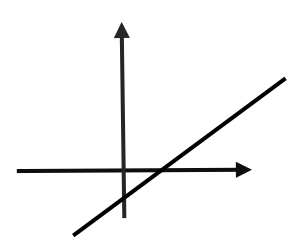
\includegraphics[width=0.2\textwidth]{D1.png} & 
    \centering \vspace{-0.3cm} \textbf{B.} La droite $d_2$ : 
    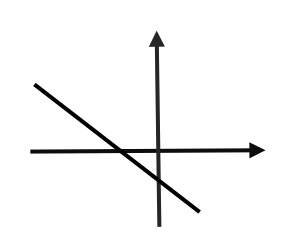
\includegraphics[width=0.2\textwidth]{D4.png} & 
    \centering \vspace{-0.3cm} \textbf{C.} La droite $d_3$ : 
    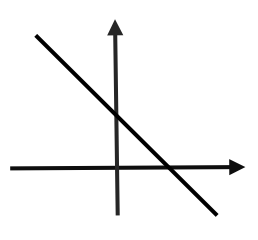
\includegraphics[width=0.2\textwidth]{D3.png} & 
    \centering \vspace{-0.3cm} \textbf{D.} La droite $d_4$ : 
    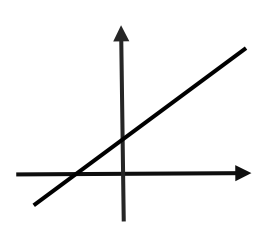
\includegraphics[width=0.2\textwidth]{D2.png} \tabularnewline
    \hline
    \end{tabular}
\end{center}

\vspace{10pt}

\textbf{Question 12 :}
\vspace{5pt}

L’épaisseur d’une feuille de papier est égale à $60 \times 10^{-3}$mm.
L’épaisseur d’une pile de 2 000 feuilles est égale à :

\begin{center}
    \renewcommand{\arraystretch}{3}
    \begin{tabular}{|m{3.4cm}|m{3.4cm}|m{3.9cm}|m{3.4cm}|}
    \hline
    \centering \vspace{-0.3cm} \textbf{A.} 120 cm & 
    \centering \vspace{-0.3cm} \textbf{B.} 12 cm & 
    \centering \vspace{-0.3cm} \textbf{C.} 12 mm & 
    \centering \vspace{-0.3cm} \textbf{D.} 62 cm \tabularnewline
    \hline
    \end{tabular}
\end{center}

\vspace{10pt}







%====================================================
%=============== DEUXIÈME PARTIE ====================
%====================================================

\begin{center}
    \textbf{DEUXIÈME PARTIE (14 points )}
\end{center}

\textbf{\underline{Exercice 1} (6 points)}

\vspace{10pt}
Léa et Benjamin possèdent tous les deux 5 000€ sur leurs comptes. Le 1\up{er} février 2020, ils décident de 
placer leur argent sur des livrets d'épargne. 

\vspace{5pt}
Léa décide de placer son argent sur un livret A et Benjamin sur un livret B.

\vspace{10pt}

\textbf{ÉTUDE DU LIVRET B}

\vspace{5pt}
Chaque année, le livret B de Benjamin lui rapporte 3\% d'intérêts. Pour tout entier $n$, On note $w_n$ l'épargne disponible 
sur le livret B à l'année $2020 + n$.

\vspace{5pt}
\begin{questions}

\question
\begin{parts}
    \part[0,5] Quelle est la valeur de $w_0$ ?
    \part[0,5] Calculer $w_1$ et interpréter ce résultat.
\end{parts}

\question[1] Exprimer $w_{n+1}$ en fonction de $w_n$. Quelle est la nature de cette suite ? Préciser 
ses éléments caractéristiques.

\question[1] Déterminer le sens de variation de $(w_n)$. Justifier votre réponse.

\end{questions}

\vspace{0.5cm}

\textbf{ÉTUDE DU LIVRET A}

\vspace{5pt}
Chaque année, le livret A de Léa lui rapporte 200€. Pour tout entier $n$, On note $u_n$ l'épargne disponible 
sur le livret A à l'année $2020 + n$.

\vspace{5pt}
\begin{questions}

\question[0,5] Calculer $u_1$, $u_2$ et $u_3$.

\question[1] Quelle est la nature de cette suite ? Donner ses éléments caractéristiques.

\question[1] Exprimer $u_n$ en fonction de $n$.

\question[0,5] En 2040, quel contrat, entre le A et le B, aura rapporté le plus d'argent ? 
On pourra utiliser la formule explicite pour les 2 suites étudiées. Justifier votre réponse.

\end{questions}

\vspace{0.5cm}

% ======================================================
\noindent
\textbf{\underline{Exercice 2} (4 points)}

\vspace{5pt}
\noindent
On considère la fonction définie sur $\mathbb{R}$ suivante :
\[
f(x) = -2x^2 + 10x - 8
\]

\begin{questions}

\question[1] Calculer l'image de 0 et de 3 par la fonction $f$.

\question[1] Montrer que pour tout réel $x$, on a : $f(x) = 2(x-1)(4-x)$.

\question[1] En déduire les racines du polynôme $-2x^2 + 10x - 8$.

\question[1] Construire le tableau de \underline{signes} de $f$.

% \question[1] En déduire les solutions de l'inéquation $f(x) \leq 0$.

\end{questions}

\vspace{1cm}

% ======================================================
\noindent
\textbf{\underline{Exercice 3} (4 points)}

\vspace{5pt}
Lors du test d'un médicament sur 300 personnes, 80 ont reçu sans le savoir un 
médicament placebo. Les effets secondaires relevés sont les suivants :

\begin{center}
    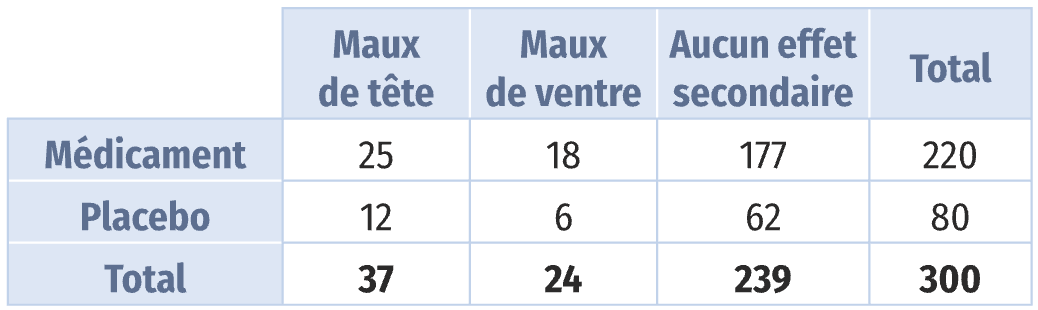
\includegraphics[width=0.6\textwidth]{tableau_medoc.png}    
\end{center}

\begin{questions}

\question[2] Calculer la fréquence conditionnelle des personnes ayant eu des maux de tête
parmi ceux qui ont pris le médicament placebo.

\question[2] \underline{FACULTATIF SI TIERS TEMPS} Calculer la fréquence marginale (en pourcentage arrondi à l'unité) 
des personnes n'ayant eu aucun effet secondaire.

\end{questions}

\vspace{0.5cm}

\begin{center}
    \textit{Fin de l'épreuve}
\end{center}

\end{document}
